\begin{figure}[h!]
	\centering
	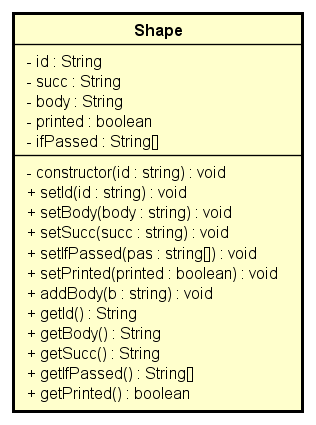
\includegraphics[scale=0.8]{res/sections/SpecificaFrontEnd/Services/Disegnetti/shape.png}
	\caption{Diagramma della classe Shape}
\end{figure}

\begin{itemize}
	\item \textbf{Descrizione:}\\
	
	\item \textbf{Utilizzo:}\\
	
	\item \textbf{Metodi:}
		\begin{itemize}
			\item \emph{-id: string}\\
    		Id della shape
    		\item \emph{-succ: string}\\
    		Elemento linkato successivo
    		\item \emph{-body: string}\\
    		Body della shape
    		\item \emph{-printed: boolean}\\
    		True se la shape è stampata
    		\item \emph{-ifPassed: String[]}\\
    		Rappresenta il codice generato
		\end{itemize}
	\item \textbf{Metodi:}
		\begin{itemize}
			\item \emph{-constructor(id: string)}\\
    		Costruttore della classe\\
    		\textbf{Parametri:}
    		\begin{itemize}
    			\item \emph{id: string}\\
    			Id della shape
    		\end{itemize}
    		\item \emph{+setId(id: string)}\\
    		etta l'id della shape\\
    		\textbf{Parametri:}
    		\begin{itemize}
    			\item \emph{id: string}\\
    			Id della shape
    		\end{itemize}
    		\item \emph{+setBody(body: string)}\\
    		Setta il body della shape\\
    		\textbf{Parametri:}
    		\begin{itemize}
    			\item \emph{body: string}\\
    			Body della shape
    		\end{itemize}
    		\item \emph{+setSucc(succ: string)}\\
    		Setta l'elemento linkato succesivamente alla shape\\
    		\textbf{Parametri:}
    		\begin{itemize}
    			\item \emph{succ: string}\\
    			Elemento successivo
    		\end{itemize}
    		\item \emph{+setIfPassed(pas: string[])}\\
    		Setta l'attributo ifPassed\\
    		\textbf{Parametri:}
    		\begin{itemize}
    			\item \emph{pas: string[]}\\
    			Nuovo valore dell'attributo
    		\end{itemize}
    		\item \emph{+setPrinted(printed: boolean)}\\
    		Setta il valore di printed\\
    		\textbf{Parametri:}
    		\begin{itemize}
    			\item \emph{printed: boolean}\\
    			Valore dell'atributo
    		\end{itemize}
    		\item \emph{+addBody(b: string)}\\
    		Aggiunge un corpo alla shape\\
    		\textbf{Parametri:}
    		\begin{itemize}
    			\item \emph{b: string}\\
    			Corpo da aggiungere
    		\end{itemize}
    		\item \emph{+getId()}\\
    		Ritorna l'attributo id della shape
    		\item \emph{+getBody()}\\
    		Ritorna l'attributo body della shape
    		\item \emph{+getSucc()}\\
    		Ritorna l'attributo succ della shape
    		\item \emph{+getIfPassed()}\\
    		Ritorna l'attributo ifPassed della shape
    		\item \emph{+getPrinted()}\\
    		Ritorna l'attributo printed della shape
    	\end{itemize}
\end{itemize}